\documentclass[]{article}

\usepackage[utf8]{inputenc}
\usepackage[spanish]{babel}
\usepackage{amsmath}
\usepackage{graphicx}
\usepackage{siunitx}
\usepackage{units}
\usepackage[margin=0.5in]{geometry}

%opening
\title{Taller 6. Flujo Continuidad y Bernoulli}
\author{Miguel A. Gomez B.}

\begin{document}

\maketitle

\section{Flujo}
%--------------------------- EJERCICIO 1
\paragraph{Ejercicio}
fluyen \SI{0,075}{\frac{\meter^3}{\second}} de agua a \SI{10}{\celsius}. ¿Cuál es el flujo másico?.
\subparagraph{Solución}
La ecuación del flujo másico es:\\
\[ \dot{m} = \dot{q} \rho \]
Donde:
\begin{itemize}
	\item $\dot{q}$ es el flujo volumétrico. Y que conocemos es de \SI{0,075}{\frac{\meter^3}{\second}}.
	\item $\rho$ es la densidad del fluído. En este caso Agua a \SI{10}{\celsius}. Es decir \SI{1000}{\frac{\kilogram}{\meter^3}}.
\end{itemize}
Por ende, al reemplazar en el sistema obtenemos:
\begin{align*}
	\dot{m} &= \left(\SI{0,075}{\frac{\meter^3}{\second}}\right)\left(\SI{1000}{\frac{\kilogram}{\meter^3}}\right)\\
			&= \SI{75}{\frac{\kilo}{\second}}
\end{align*}

Por lo tanto el flujo másico será $\SI{75}{\frac{\kilo}{\second}}$.


%--------------------------- EJERCICIO 2
\paragraph{Ejercicio}
Un líquido refrigerante  $S=1,08$ fluye dentro de una tubería de $\frac{1}{2}$ in de diámetro de cobre tipo K. Si la velocidad de flujo es de \SI{0,5}{\frac{\meter}{\second}} ¿Cuál es el flujo volumétrico y el flujo másico?

\subparagraph{Solución}
Mediante la ecuación del flujo másico podemos obtener el flujo volumétrico
\[ \dot{m} = \dot{q} \rho \]
\[ \dot{q} = \frac{ \dot{m} }{ \rho } \]
Existe una segunda ecuación para hallar el flujo másico
\[ \dot{m} = \rho A \bar{V} \]
Donde:
\begin{itemize}
	\item $\rho$ es la densidad del fluído. En este caso la obtendremos mediante la ecuación de la gravedad específica
	
	\[ S = \frac{ \rho_x } { \rho_{H_{2}O} }\]
	
	Sabemos que la densidad del agua es de \SI{998}{ \frac{ \kilogram } { \meter^3 } }, por ende:
	
	\begin{align*}
		\rho_x &= S \rho_{H_{2}O}\\
		       &= (1,08)\left(\SI{998}{ \frac{ \kilogram } { \meter^3 } }\right)\\
		       &= \SI{1077} { \frac{ \kilogram } { \meter^3 } }
	\end{align*}

	
	\item $A$ es el flujo de área para la tubería y que es
	\[
		A = \SI{1,515e-3}{ft^2} = \SI{1,407e-4}{\meter^2}
	\]
	\item $\bar{V}$ es un valor conocido de \SI{0,5}{\frac{\meter}{\second}}.
\end{itemize}

Luego únicamente debemos reemplazar los valores encontrados en cada una de las ecuaciones.

\subparagraph{Flujo másico}

\begin{align*}
	\dot{m} &= \rho A \bar{V}\\
	        &= \left(\SI{1077} { \frac{ \kilogram } { \meter^3 } }\right) 
	           (\SI{1,407e-4}{\meter^2})
	           \left(\SI{0,5}{\frac{\meter}{\second}}\right)\\
	        &\approx \SI{0,075} { \frac{ \kilogram } { \second } }\\
\end{align*}

Por lo tanto, el flujo másico será \SI{0,075} { \frac{ \kilogram } { \second } }.

\subparagraph{Flujo volumétrico}

\begin{align*}
	\dot{q} &= \frac{ \dot{m} }{ \rho }\\
	        &= \frac{ \SI{0,075} { \frac{ \kilogram } { \second } } } 
	                { \SI{1077} { \frac{ \kilogram } { \meter^3 } } }\\
	        &\approx \SI{ 6,97e-5 }{ \frac{ \meter^3 } { \second } }
\end{align*}

Por lo tanto, el flujo volumpetrico será \SI{ 6,97e-5 }{ \frac{ \meter^3 } { \second } }.

%--------------------------- EJERCICIO 3

\paragraph{Ejercicio}
Un horno necesita \SI{1200}{\frac{lb_m}{\hour}} de aire para obtener combustión eficiente. Si el aire tiene un peso específico de \SI{0,062}{\frac{lb_f}{ft^3}} ¿Cuál es el flujo volumétrico?

\subparagraph{Solución}
Sabemos que:

\[ \dot{q} = \frac{ \dot{m} }{ \rho } \]

Tenemos que $\dot{m} = \SI{1200}{\frac{lb_m}{\hour}}$ y que es equivalente a:
\begin{align*}
	\dot{m} &= \left( \SI{1200}{\frac{lb_m}{\hour}} \right)
			   \left(
			   	\SI{0,453}{\frac{\kilogram}{lb_m}}
			   \right)\\
	        &= \SI{543,6}{\frac{\kilogram}{\hour}} \left( \frac{1}{3600}\SI{}{\frac{\hour}{\second}} \right)\\
	        &= \SI{0,151}{\frac{\kilogram}{\second}}
\end{align*}

También tenemos que $\gamma$ representa el peso específico y equivale a \SI{0,062}{\frac{lb_f}{ft^3}}, se realiza la conversión:
\[ \gamma = \left( \SI{ 0,062 }{\frac{ lb_f } { ft^3  } } \right)
\left( \SI{ 157,1 }
{ 
	\frac {
		\frac{ \newton }{ \meter^3 }
	}  
	{ 
		\frac { lb_f } { ft^3 } 
	}
} 
\right)
\approx \SI{9,74}{\frac{ \newton }{ \meter^3 }}
\]

Sabemos que 

\[ \gamma = \rho g \rightarrow \rho = \frac{ \gamma } { g } \]

\begin{itemize}
	\item $\rho$ representa la densidad del fluido.
	\item $g$ es la gravedad y equivale a \SI{9,81}{\frac{\meter} {\second^2}}.
\end{itemize}

Hallamos $\rho$:
\begin{align*}
	\rho &= \frac{ \gamma } { g }\\
		 &= \frac { \SI{9,74}{\frac{ \newton }{ \meter^3 }} }
		 		  { \SI{9,81}{\frac{\meter} {\second^2}} }\\
		 &\approx \SI{0,992}{ \frac{\kilogram}{\meter^3} }
\end{align*}

Ahora es posible hallar $\dot{q}$:

\begin{align*}
	\dot{q} &= \frac{ \dot{m} }{ \rho }\\
	        &= \frac{ \SI{0,151}{\frac{\kilogram}{\second}} }
	                { \SI{0,992}{\frac{\kilogram}{\meter^3}} }\\
	        &\approx \SI{0,152}{\frac{\meter^3}{\second}}
\end{align*}

Por lo tanto el flujo volumétrico $\dot{q}$ es $\approx \SI{0,152}{\frac{\meter^3}{\second}}$

\newpage

\section{Continuidad}

%--------------------------- EJERCICIO 4

\paragraph{Ejercicio}
Si la velocidad de un líquido es de \SI{1,65}{\frac{ft}{\second}} en una tubería de \SI{12}{in} de diámetro interno ¿Cuál es la velocidad de un chorro que sale de una tubería de \SI{3}{in} de diámetro interno?

\subparagraph{Solución}
Definimos:

\begin{itemize}
	\item $\bar{V}_i$ como la velocidad inicial del fluido igual a $\SI{1,65}{\frac{ft}{\second}}$.
	\item $\oslash_i$ como el diámetro inicial de la tubería e igual a \SI{12}{in} que equivale a \SI{1}{ft}.
	\item $\oslash_f$ como el diámetro final de la tubería e igual a \SI{3}{in} y que en pies equivale a \SI{0,25}{ft}.
	\item $\bar{V}_f$ cómo la velocidad final y es el valor que quermos hallar.
\end{itemize}

Derivado de la ley de continuidad tenemos que

\[ A_1 \bar{V}_1 = A_2 \bar{V}_2 \]

donde los $A_n$ representan las áreas de la tubería con flujo continuo y los $\bar{V}_n$ representan las velocidades de los flujos para las secciones $n$ de la tubería. Utilizando esto en nuestro problema tenemos

\[ A_i \bar{V}_i = A_f \bar{V}_f \]

Luego,

\[ \frac{A_i \bar{V}_i} { A_f } = \bar{V}_f \]

Dado que las tuberías son cilindricas, los $A_n$ se convierten en hallar el área de dos círculos:

\[ A_i = \frac{\pi (\oslash_i)^2}{4} = \frac{\pi (\SI{1}{ft})^2}{4} = \frac{\pi}{8}\SI{}{ft^2} \]
\[ A_f = \frac{\pi (\oslash_f)^2}{4} = \frac{\pi (\SI{0,25}{ft})^2}{4} = \frac{\pi}{64}\SI{}{ft^2} \]

Ahora hallamos $\bar{V}_f$:

\begin{align*}
	\bar{V}_f &= \frac{A_i \bar{V}_i} { A_f }\\
	          &= \frac{\frac{\pi}{8}\SI{}{ft^2} (\SI{1,65}{\frac{ft}{\second}})} 
	                  {\frac{\pi}{64}\SI{}{ft^2}}
	           =  \frac{1}{8}\left(\SI{1,65}{\frac{ft}{\second}}\right)\\
	          &\approx \SI{206,05e-3}{\frac{ft}{\second}} 
\end{align*}

Por lo tanto la velocidad en esa sección de la tubería será de $\approx$ \SI{206,05e-3}{\frac{ft}{\second}}.

%--------------------------- EJERCICIO 5

\paragraph{Ejercicio}
Una tubería de \SI{150}{\milli\meter} de diámetro interno conduce \SI{0,072}{\frac{\meter^3}{\second}} de agua. La tubería se divide en dos ramales. Si la velocidad de la tubería de \SI{50}{\milli\meter} es de \SI{12}{\frac{\meter}{\second}} ¿Cuál es la velocidad de la tubería de \SI{100}{\milli\meter}?

\begin{figure}[h!]
	\centering
	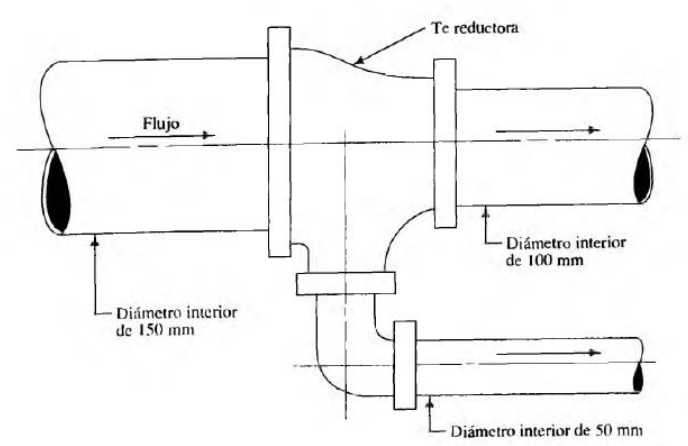
\includegraphics[width=0.9\linewidth]{img/1.png}
	\caption{Imagen ejemplo del ejericicio.}
	\label{fig:io_1}
\end{figure}

Definimos:

\begin{itemize}
	\item $\oslash_1$ como la tubería que tiene \SI{150}{\milli\meter} de diámetro.
	\item $\dot{q}$ como el flujo volumétrico inicial y que lleva \SI{0,072}{\frac{\meter^3}{\second}} de agua.
	\item $\oslash_{50}$ como la tubería que tiene \SI{50}{\milli\meter} de diámetro.
	\item $\bar{V}_{50}$ la velocidad del fluído en la tubería de \SI{50}{\milli\meter} y equivale a \SI{12}{\frac{\meter^3}{\second}}.
	\item $\oslash_{100}$ como la tubería que tiene \SI{100}{\milli\meter} de diámetro.
\end{itemize}

Siendo $\dot{q}_{50}$ y $\dot{q}_{100}$ los flujos que van por cada una de las tuberías de 50 y 100 milímetros, por la ley de continuidad sabemos que:

\[ \dot{q} = \dot{q}_{50} + \dot{q}_{100} \]

Adicionalmente

\[ \dot{q}_n = A_n \bar{V}_n \]

por ello:

\[
	\dot{q}_{50} = A_{50}\bar{V}_{50}
\]
Luego,
\begin{align*}
	A_{50} &= \frac{\pi (\oslash_{50})^2}{4}\\
	       &= \frac{\pi (\SI{50e-3}{\meter})^2}{4}\\
	       &\approx \SI{1,963e-3}{\meter^2}
\end{align*}

Hallamos $\dot{q}_{50}$:

\begin{align*}
	\dot{q}_{50} &= A_{50} \bar{V}_{50}\\
				 &= \left( \SI{1,963e-3}{\meter^2} \right)
				    \left( \SI{12}{\frac{\meter}{\second}} \right)\\
				 &\approx \SI{0,024}{\frac{\meter^3}{\second}}
\end{align*}

Al reemplazar el la ecuación de flujos tenemos:

\begin{align*}
	\dot{q}_{100} &= \dot{q} - \dot{q}_{50}\\
				  &= \SI{0,072}{\frac{\m^3}{s}} - \SI{0,024}{\frac{\meter^3}{\second}}\\
				  &= \SI{0,048}{\frac{\meter^3}{\second}}
\end{align*}

$\dot{q}_{100}$ también se puede expresar como

\[ \dot{q}_{100} = A_{100} \bar{V}_{100} \rightarrow \bar{V}_{100} = \frac{\dot{q}_{100}}{A_{100}} \]

Hallamos $A_{100}$:

\begin{align*}
	A_{100} &= \frac{\pi (\oslash_{100})^2}{4}\\
	        &= \frac{\pi (\SI{100e-3}{\meter})^2}{4}\\
	        &\approx \SI{7,853e-3}{\meter^2}
\end{align*}

finalmente podemos hallar $\bar{V}_{100}$:

\begin{align*}
	\bar{V}_{100} &= \frac{\dot{q}_{100}}{A_{100}}\\
	              &= \frac{\SI{0,048}{\frac{m^3}{s}}}
	                {\SI{7,853e-3}{\meter^2}}\\
	              &\approx \SI{6,112}{\frac{\meter}{\second}}
\end{align*}

De modo que la velocidad en la túbería de 100 milímetros será de \SI{6,112}{\frac{\meter}{\second}}.


%--------------------------- EJERCICIO 6

\paragraph{Ejercicio}
Si \SI{2000}{\frac{\liter}{\minute}} de agua fluyen a través de una tubería de \SI{300}{\milli\meter} de diámetro que después se reduce a \SI{150}{\milli\meter}, calcule la velocidad promedio del flujo en cada tubería.

\subparagraph{Solución}
Tenemos:
\begin{itemize}
	\item El flujo volumétrico $\dot{q}$ que equivale a \SI{2000}{\frac{\liter}{\minute}} y que equivale a \SI{2}{\frac{\meter^3}{\minute}}.
	\item El diámetro inicial de la tubería $\oslash_{i}$ y que equivale a \SI{300e-3}{\meter}.
	\item El diámetro final de la tubería $\oslash_{f}$ y que equivale a \SI{150e-3}{\meter}.
\end{itemize}

Por la ecuación del flujo volumétrico sabemos que

\[
	\dot{q} = A \bar{V} \rightarrow \bar{V} = \frac{\dot{q}}{A}
\]

Definimos $A_{i}$ y $A_f$ como los valores de las áreas de las  tubería inicial y final

\[ 
	A_n = \frac{\pi\oslash_n}{4}
\]

Las hallamos con la formula anterior

\begin{align*}
	A_i &= \frac{ \pi(\oslash_i)^2 }{4}\\
	    &= \frac{ \pi(\SI{300e-3}{\meter})^2 }{4}\\
   	    &\approx \SI{0,07}{\meter^2}
\end{align*}

\begin{align*}
	A_f &= \frac{ \pi(\oslash_f)^2 }{4}\\
		&= \frac{ \pi(\SI{150e-3}{\meter})^2 }{4}\\
		&\approx \SI{0,017}{\meter^2}
\end{align*}


Luego ahora es posible hallar las velocidades:

\begin{align*}
	\bar{V}_i &= \frac{\dot{q}}{A_i}\\
		   	  &= \frac{\SI{2}{\frac{\meter^3}{\minute}}}{\SI{0,07}{\meter^2}}\\
		   	  &\approx \SI{28,571}{\frac{\meter}{\minute}}
\end{align*}

\begin{align*}
	\bar{V}_f &= \frac{\dot{q}}{A_f}\\
			  &= \frac{\SI{2}{\frac{\meter^3}{\minute}}}{\SI{0,017}{\meter^2}}\\
			  &\approx \SI{117,647}{\frac{\meter}{\minute}}
\end{align*}

Por lo tanto para las condiciones del problema las velocidades del fluido en cada una de las tuberías será de \SI{28,571}{\frac{\meter}{\minute}} y \SI{117,647}{\frac{\meter}{\minute}}.

\newpage

\section{Bernoulli}

%--------------------------- EJERCICIO 7

\paragraph{Ejercicio}
Por la tubería de la figura fluyen \SI{0,11}{\frac{\meter^3}{\second}} de gasolina ($S=0.67$) si la presión antes de la reducción es de \SI{415}{\kilo\pascal}, calcule la presión de la tubería de \SI{75}{\milli\meter} de diámetro.

\begin{figure}[h!]
	\centering
	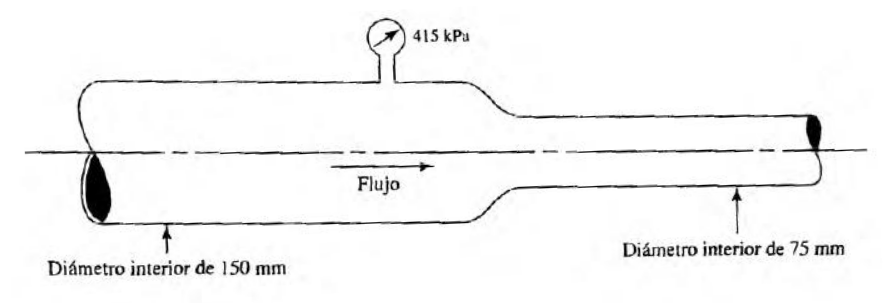
\includegraphics[width=0.9\linewidth]{img/2.png}
	\caption{Imagen ejemplo del ejericicio.}
	\label{fig:io_2}
\end{figure}

\subparagraph{Solución} Utilizamos la ecuación de bernoulli

\[ \frac{\rho(\bar{V}_i)^2}{2} + \rho g h_1 + P_1 = \frac{\rho (\bar{V}_f)^2}{2} + \rho g h_2 + P_2 \]

Para éste problema no existen cambios de altura por lo que $h_1$ y $h_2$ pueden asumirse como 0 y tendríamos ahora

\[ \frac{\rho(\bar{V}_1)^2}{2} + P_1 = \frac{\rho (\bar{V}_2)^2}{2} + P_2 \]

Dónde:

\begin{itemize}
	\item $P_1$ es la presión inicial y equivale a \SI{415}{\kilo\pascal}.
	\item $\dot{q}$ es el flujo volumétrico y equivale a \SI{0,11}{\frac{\meter^3}{\second}}.
	\item $\bar{V}_1$ y $\bar{V}_2$ son las velocidades en la tubería antes y después de la reducción. es posible obtenerlas con las ecuaciones de continuidad.
	\begin{align*}
		\bar{V}_1 &= \frac{\dot{q}}{A_1}\\
		          &= \frac{\SI{0,11}{\frac{\meter^3}{\second}}}
		                  {
		                  	\frac{\pi(\SI{150e-3}{\meter})^2}{4}
		                  }\\
	              &\approx \SI{6,224}{\frac{\meter}{\second}}
	\end{align*}
	\begin{align*}
		\bar{V}_2 &= \frac{\dot{q}}{A_2}\\
				  &= \frac{\SI{0,11}{\frac{\meter^3}{\second}}}
						  {
						  	\frac{\pi(\SI{75e-3}{\meter})^2}{4}
						  }\\
		&\approx \SI{24,899}{\frac{\meter}{\second}}
	\end{align*}
	\item $\rho$ es la densidad del fluido que se puede obtener mediante la fórmula de la gravedad específica:
	\[ S = \frac{\rho_x}{\rho_{H_{2}O}} \rightarrow \rho_x = S \rho_{H_{2}O} \]
	$\rho_{H_{2}O}$ es un valor conocido en condiciones ideales y equivale a \SI{998}{\frac{\kilogram}{\meter^3}}.
	\begin{align*}
		\rho_x &= S \rho_{H_{2}O}\\
		       &= \left( 0,67 \right) \left( \SI{998}{\frac{\kilogram}{\meter^3}} \right)\\
		       &= \SI{668,66}{\frac{\kilogram}{\meter^3}}
	\end{align*}
\end{itemize}

Ahora reorganizamos los términos de la ecuación inicial para obtener el valor de $P_2$, así:

\[ \frac{\rho(\bar{V}_1)^2}{2} + P_1 = \frac{\rho (\bar{V}_2)^2}{2} + P_2 \]

\[ \frac{\rho(\bar{V}_1)^2}{2} + P_1 - \frac{\rho (\bar{V}_2)^2}{2} = P_2 \]

Reorganizando el sistema y evaluando con los valores conocidos obtenemos:

\begin{align*}
	P_2 &= \frac{\rho}{2} \left[(\bar{V}_1)^2 - (\bar{V}_2)^2 \right] + P_1\\
		&= \left( \frac{\SI{668,66}{\frac{\kilogram}{\meter^3}}}{2} \right) 
		   \left[ 
		   			\left(\SI{6,224}{\frac{\meter}{\second}}\right)^2 - 
		   			\left(\SI{24,899}{\frac{\meter}{\second}}\right)^2
		   \right] + \SI{415e3}{\pascal}\\
		&\approx \SI{220,68}{\kilo\pascal}
\end{align*}

Por lo tanto la presión en la segunda sección de la tubería en donde se reduce el diámetro a \SI{75}{\milli\meter} será cercana a \SI{220,68}{\kilo\pascal}.

\newpage

%--------------------------- EJERCICIO 8

\paragraph{Ejercicio}
Calcule el flujo volumétrico de agua a \SI{5}{\celsius} que pasa por el sistema ilustrado en la figura.

\begin{figure}[h!]
	\centering
	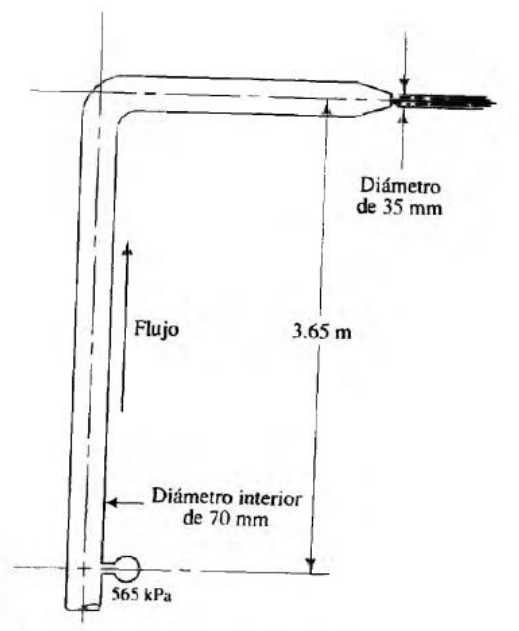
\includegraphics[width=0.5\linewidth]{img/3.png}
	\caption{Imagen ejemplo del ejericicio.}
	\label{fig:io_3}
\end{figure}


%--------------------------- EJERCICIO 9

\paragraph{Ejercicio}
Desde una tubería estándar de acero de \SI{1}{in} cedula 40, fluye keroseno con peso específico de \SI{50}{\frac{lb}{ft^3}} a razón de \SI{10}{\frac{gal}{\min}} hacia otra tubería estándar también de acero de \SI{2}{in} cedula 40. Calcule la diferencia en la presión de los dos tubos.

%--------------------------- EJERCICIO 10

\paragraph{Ejercicio}
Para el sistema mostrado en la figura calcule la presión a la salida si la velocidad de agua a \SI{25}{\celsius} es de \SI{15}{\frac{\meter}{\second}}.

\begin{figure}[h!]
	\centering
	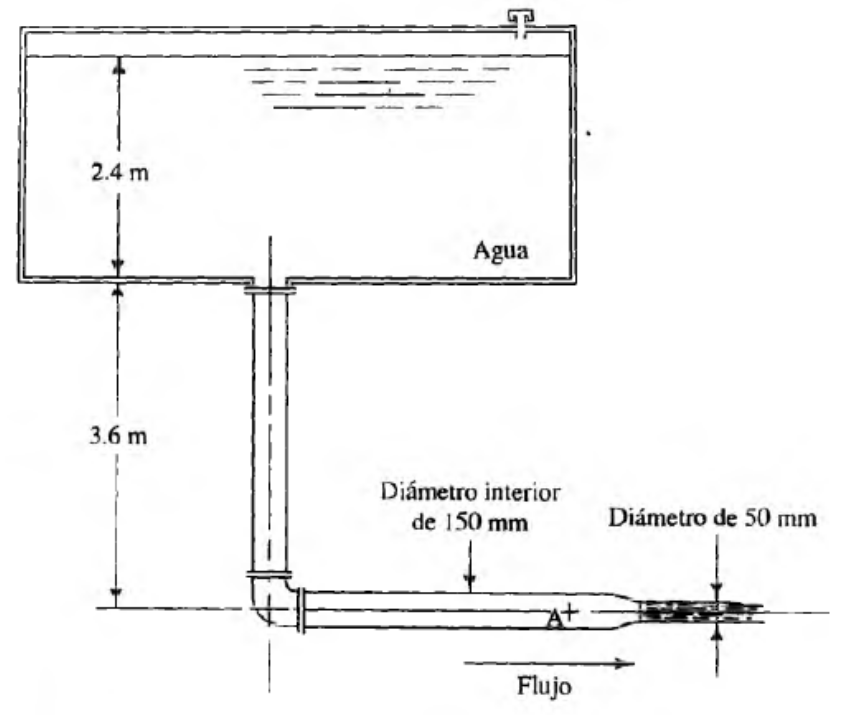
\includegraphics[width=0.7\linewidth]{img/4.png}
	\caption{Imagen ejemplo del ejericicio.}
	\label{fig:io_4}
\end{figure}

\end{document}